\clearpage
\section{Neuroevolution}

In this section we discuss \textit{neuroevolution}, which is a application of the genetic algorithm discussed in Section ? is used to train a neural network.

\subsection{Overview}

The key idea behind neuroevolution is to use neural nets as the chromosomes in a genetic algorithm. The weights of the connections between neurons (and potentially the connections themselves) play the part of the genes. Neuroevolution is particularly suited to problems where labelled input/output pairs do not exist, but it is still relatively easy to assess the performance of a solution at the end of a training run via a fitness function. The lack of labelled data at each time step makes it impossible to train the network using backpropagation, but the genetic algorithm approach still works because the fitness of each neural net only needs to be calculated at the end of an epoch. Implementing the underlying neural networks is straightforward under neuroevolution, since the approach only requires feed forward networks.

\begin{figure}[!htbp]
    \centering
    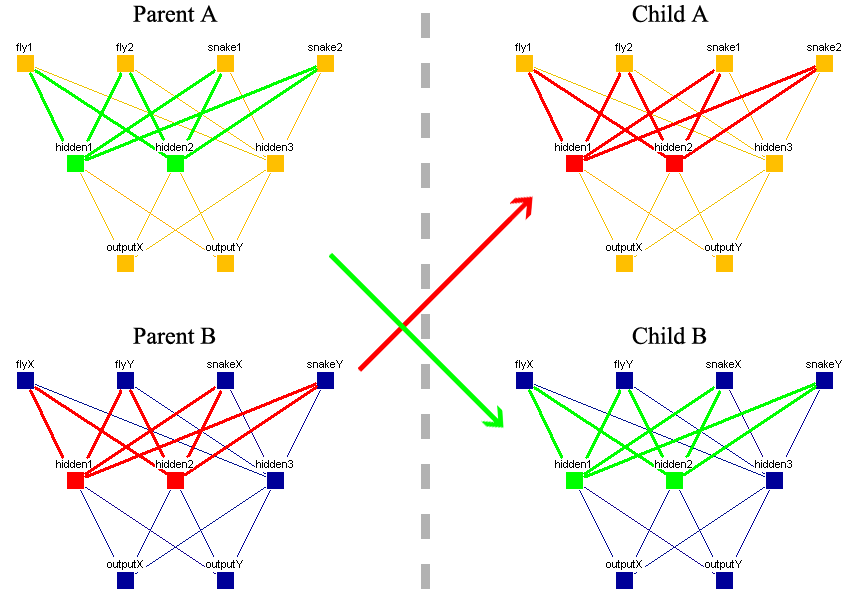
\includegraphics[scale=0.6]{Figs/Crossover.png}
    \caption{A crossover operation applied to neural networks. Here, there are two genes crossed over.}
    \label{fig:netCrossover}
\end{figure}

Neuroevolution generally performs best if each neuron and its input weights are treated as a single, cohesive gene. This is because a neuron's input weights are generally fine-tuned in relation to each other in a well-performing network, so crossing over halfway between weights will likely ruin the neuron's precise configuration. For example, the crossover depicted in Figure \ref{fig:netCrossover} involves \textit{two} genes, each consisting of four weights. Mutation does not work this way however; the weights are perturbed individually.

\subsection{Neuroevolution in Our Game}
Automating the steering of the frog in our game seemed like a perfect opportunity to apply neuroevolution. Our aim was to train a neural network that, given a set of real-time game data (such as the positions of the nearest flies, snakes, obstacles and lakes), would output an appropriate $(x, y)$ steering for the frog. It would be difficult to use the backpropagation for training such a network, because it is not clear what constitutes a ``good'' steering vector at each instant in the game.\footnote{It would be possible to record a set of data from human play and train the frog to mimic such play, but we wanted the frog to learn for itself.} However, it is relatively easy to assess the performance of a frog after some time has passed by considering how many flies it caught and how many times it was hurt by snakes.

\subsubsection{Network Architecture}
As we alluded to above, the inputs our networks receive are the $(x, y)$ positions of the nearest flies, snakes, obstacles and lakes. Our implementation is dynamic so that the number of nearest objects of each type can be modified easily or omitted. This was so that we could experiment with training simple tasks first (e.g. catching stationary flies with no predators or obstacles) then increase the difficulty as we discovered what the frogs were capable/incapable of learning.

The inputs are calculated relative to the frog; i.e. the vector from the frog to each object is used, not the object's world co-ordinates. It is common to also normalise rotations to the frog's co-ordinate system, but we experimented with this approach and found that it was not of much help. The problem with taking the frog's rotation into account is that the frog's rotation does not particularly matter in our game. The frog's turn speed is so fast that it does not matter if, for example, the frog is facing a snake or has its back turned (see Figure \ref{fig:NormalisationProblem}). These are presented as different inputs if the input is normalised, but the frog's behaviour should probably be the same either way.

\begin{figure}[!htbp]
    \centering
    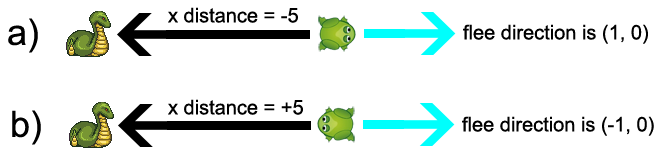
\includegraphics[scale=0.6]{Figs/NormalisationProblem.png}
    \caption{a) ??? b) ???}
    \label{fig:NormalisationProblem}
\end{figure}

Our ultimate approach makes full use of the roational symmetry of the game. We present the input multiple times with different rotations applied, calculate the outputs, then un-rotate the outputs and calculate the average steering.

One final note for the neural net input is that using the vector differential directly is not a good idea. It means that the closer and object gets, the weaker the signal it sends!

\begin{align}
\text{\textit{Input magnitude}} = e^{-k\|V\|}
\end{align}

where $V$ is the vector to the object and $k$ is a constant that controls dampening (equal to 10 in our implementation)

We chose to use a single hidden layer for simplicity, because in general the more complex the architecture, the longer the net takes to train (whether via backpropagation or evolution). (See figure to see how complex it is!) For the same reason we do not evolve connections, just weights. Normally neural nets squash input between (0, 1) but that doesn't make sense for us because an object could be to the left (-ve) or right (+ve) for example. Instead we squashed to (-1, 1). Don't apply a bias to this because it wouldn't make sense! Instead we maintain a weight that controls the gradient (sharpness of the rise).

For output, note that everything is continuous! This was one of the coolest things about our approach. We didn't just have four outputs representing strategies.

\subsubsection{Fitness function}

Say what it was!

\subsubsection{Challenges}

In this section we discuss some of the challenges that...

\subsubsection{Smart, Yet Undesirable Behaviour}

A major problem we encountered was that the frogs often found a ``good'' solution in terms of yielding high fitness, but the behaviour of the best performing frogs was not what we wanted  or expected. The below are just some examples:\\

\hspace*{-0.27in}
\begin{tabular}
{|p{11cm}|p{6.5cm}|}
\hline
\textbf{Problem} & \textbf{Solution}\\
\hline
If the training pen contained many flies and the flies were configured to move around with a ``wander'' steering behaviour, the frogs only learnt to avoid the snakes because chances were that they would catch several flies by pure chance. The frogs that were slightly biased to target the flies tended to get hit slightly more often too, which cancelled out the advantage. If there were too few flies then funnily enough the same thing happened, since there was not enough positive reinforcement for the frogs when they caught flies. & Making the flies stationary during training so that the frogs that deliberately targeted them got more of an advantage. Finely tuning the number of flies in the training pen and the relative sizes of the reward for catching a fly and the punishment for being hit by a snake.\\
\hline
Since the punishment for being hit by a snake is much larger than the reward for catching a fly, the frogs rightly learnt how to protect themselves first. Unfortunately, the best way to do this is to run into a lake and stay there! Once the entire population learnt this behaviour, learning stagnated because the frogs were never leaving the lake and had little opportunity to learn about the reward available through catching flies. & Introducing a ``water camping'' penalty to the fitness function. If the frogs are already full on water but continue to stay in a lake, their score is gradually decremented. (Although there is a grace period so that frogs do not have to leave immediately after topping up.)\\
\hline
Originally the training runs were fairly short (20 seconds long), but this was not long enough for poor behaviours to be exposed. For example, frogs that only targeted flies and disregarded the snakes would tend to rank first every time, because with a population size of around 50, one of the frogs would tend to get a favourable run where the snakes wandered away from the nearby flies. This encouraged excess aggression. & Increasing the time limit to 2 minutes per training run and using the same fly distribution for each pen. The fly distribution is still randomised at the start of each epoch, but the distribution is shared. Also using ranked roulette instead of proportional (?)\\
\hline
\end{tabular}

\subsubsection{Training Time}
As discussed in the third problem above, each training run needed to be reasonably long in order for the genetic algorithm to work properly. However, we found that it generally took around 1,500 epochs for the frogs' learning to start tapering off (see Figure ? later). For a population size of 40 (which is fairly typical in these types of experiments), this would have taken an extremely long time to complete! Our first measure to combat this was fairly obvious -- we increased the Unity time scale to speed up the training runs. We found that a speed up factor of around 3 -- 4 was appropriate (at higher speeds Unity became jerky). Our second measure was to clone the training pens (see Figure \ref{fig:TrainingPens}). With eight indentical pens, a population size of 40 only required 5 batches of frogs per epoch. We could have created even more pens, but Unity was taking a long time to launch the scene with so many resources loaded at once.

\begin{figure}[!htbp]
    \centering
    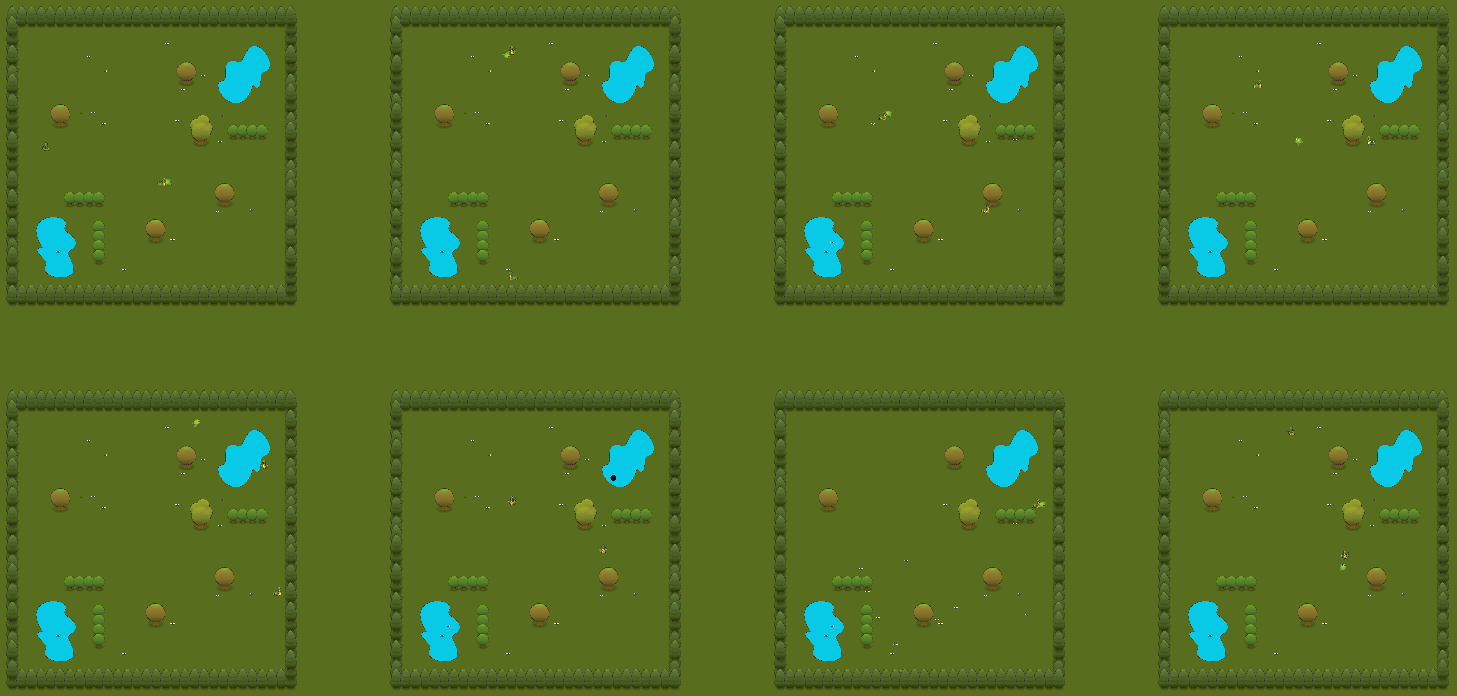
\includegraphics[scale=0.3]{Figs/TrainingPens.png}
    \caption{???}
    \label{fig:TrainingPens}
\end{figure}

\subsubsection{Obstacle Avoidance}
In the original game, the frog was controlled by mouse clicks and automatically avoided obstacles via A* (and a few additional tricks to avoid corner collisions). This time the frog was controlled by a neural network, which for out network was essentially just a type of steering behaviour. This created a problem, because A* and steering behaviours do not really gel. A* requires a goal note, but steering behaviours only provide a direction of travel, not a distance. Our solution to this problem was to modify the obstacle avoidance technique that the flies used in our first assignment so that the frogs could use it as well. This means that the frog is no longer capable of navigating mazes, so we had to ensure that the maps we used for training and the actual game did not include any ``bowl'' shapes that would trap the frog.

\subsubsection{Shooting Bubbles}
We wanted our frog to be able to shoot bubbles after filling up on water in the lakes, but we decided that having the frog learn to shoot from scratch would be too difficult (given the time limits) since opportunities to fire on snakes are limited and the overall plan of (obtain water -- approach snake -- fire bubble at correct angle) is quite a complex one, especially given that the frogs generally learn to avoid snakes. Our solution was to simply make the frog fire directly at snakes whenever they are within a certain range and the frog's water level allows it. We made it so that the shot range was an additional gene in the frog chromosome, so the frogs learned when to shoot, but not how to shoot.

[TO DO: Mention representation of bubbled snakes!]

\subsection{Outcome}
In the course of all our experiments, we found that the frogs generally learned tasks in a particular order. Since the fitness loss from being hit by a snake was far more than the benefit from catching a fly, the frogs learned the art of self preservation first. Before we added the lakes, this meant fleeing in the opposite direction from snakes. After we added the lakes, this meant diving straight into the lakes at the start of each training run. After learning self preservation, the frogs that had a tendency to catch more flies (or to leave the lake, after we added the ``water camping'' penalty) gradually became more and more dominant. Their behaviour gradually became more daring when flies were close to the snakes, and their flee patterns became much slipperier!

Given that we did not pre-program any behaviour for the frogs (besides cheating with the water bubbles), and the output of the neural nets was simply a steering (not just a selection between different behaviours), we were very happy with the performance of the frogs. Aside from our qualitative assessment that the frogs appeared to become much more intelligent during training, we were able to confirm that the genetic algorithm worked in a scientific sense by plotting the total population fitness versus epoch (see Figure ?)\\

INSERT FIGURE\\

There was a lot of variance in the fitness from epoch to epoch due to the random spawn locations of the flies, but there was a noticeable increase in performance until around epoch 1,500. The population fitness reach a peak of ?, corresponding to an average fitness of ? per frog, which is equivalent to ? (some number of flies).